\subsection{Tipo de entidad Titulación}

   \begin{description}

   \item[Definición] Se refiere al objeto del mundo real: \emph{``Conjunto de
        materias cuya superación supone la obtención de un título académico''}.

   \item[Características] La entidad presenta las siguientes características:
      \begin{itemize}
         \item \textbf{Nombre:} Titulación.
         \item \textbf{Tipo:} Fuerte.
         \item \textbf{Número de atributos:} 2.
         \item \textbf{Atributo/s identificador/es principal/es:} id\_titulacion.
         \item \textbf{Atributo/s identificador/es alternativo/s:} nombre\_titulacion
         \item \textbf{Atributo/s heredado/s:} -
      \end{itemize}

   \item[Diagrama]
   \item \begin{figure}[h!]
            \begin{center}
            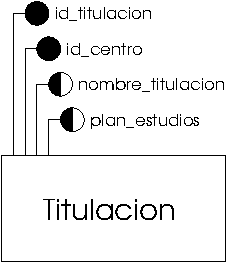
\includegraphics[]{07.Modelo_Entidad-Interrelacion/7.2.Analisis_Entidades/diagramas/titulacion.pdf}
            \caption{Diagrama de la entidad Titulación}
            \end{center}
         \end{figure}

   \item[Descripción de los atributos] La entidad presenta los siguientes
   atributos:

   \begin{itemize}
    \item \textbf{id\_titulacion}
      \begin{itemize}
         \item \textbf{Definición:} Código que sirve como número identificativo
         para cada titulación dentro del sistema.
         \item \textbf{Dominio:} Números naturales.
         \item \textbf{Carácter:} Obligatorio.
         \item \textbf{Ejemplo práctico:} 3.
         \item \textbf{Información adicional:} El dato lo genera el sistema
         cuando el administrador introduce la titulación en el sistema.
         Es la clave primaria.
      \end{itemize}
   \item \textbf{nombre\_titulacion}
      \begin{itemize}
         \item \textbf{Definición:} Denominación de una titulación dentro del sistema.
         \item \textbf{Dominio:} Conjunto de caracteres alfanuméricos.
         \item \textbf{Carácter:} Obligatorio.
         \item \textbf{Ejemplo práctico:} Ingeniería Técnica en Informática de Gestión.
         \item \textbf{Información adicional:} El dato lo proporciona el administrador en el momento de introducir la titulación en el sistema. Es la clave alterna
      \end{itemize}
   \end{itemize}

   \item[Ejemplo práctico]

   \item \begin{center}
            \begin{tabular}{ | l | l | }
            \hline
            \multicolumn{2}{ | c | }{\textbf{Tipo de entidad Titulación}} \\
            \hline
            id\_centro & 3 \\
            \hline
            nombre\_centro & Ingeniería Técnica en Informática de Gestión \\
            \hline
            \end{tabular}
         \end{center}
   \end{description}
